\begin{figure}[H]
    \centering
    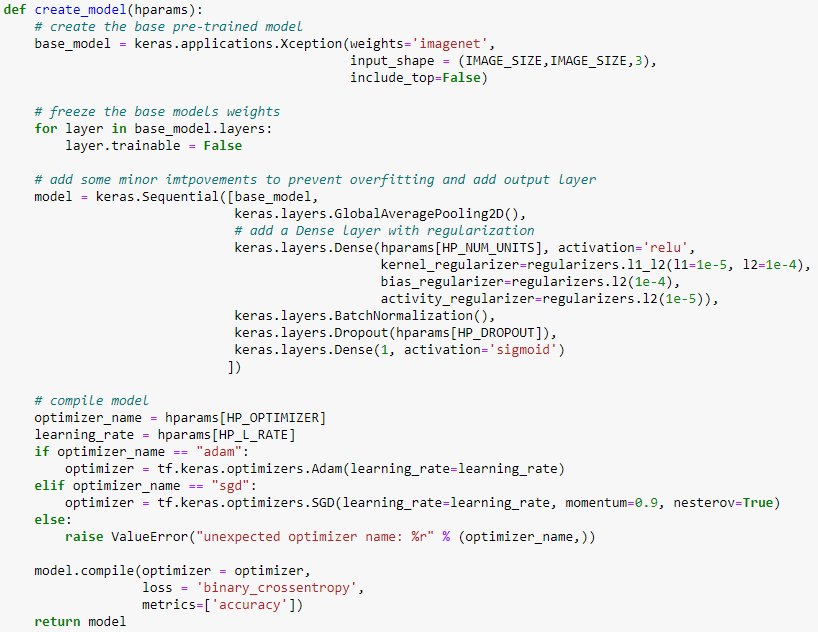
\includegraphics[width=\textwidth]{figures/xception-improvement-1.png}
    \caption{Freezing the base models trainable weights.}
    \label{fig:xception-improvement-1}
\end{figure}
\begin{figure}[H]
    \centering
    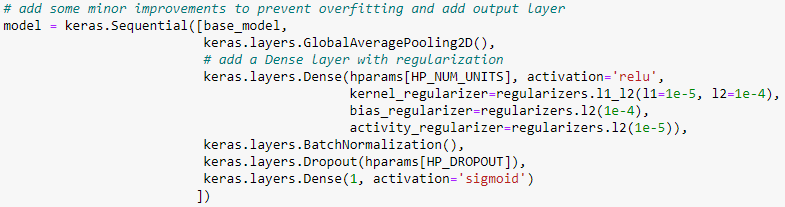
\includegraphics[width=\textwidth]{figures/xception-improvement-2.png}
    \caption{Adding regularisers to the Dense layer.}
    \label{fig:xception-improvement-2}
\end{figure}
\begin{figure}[H]
    \centering
    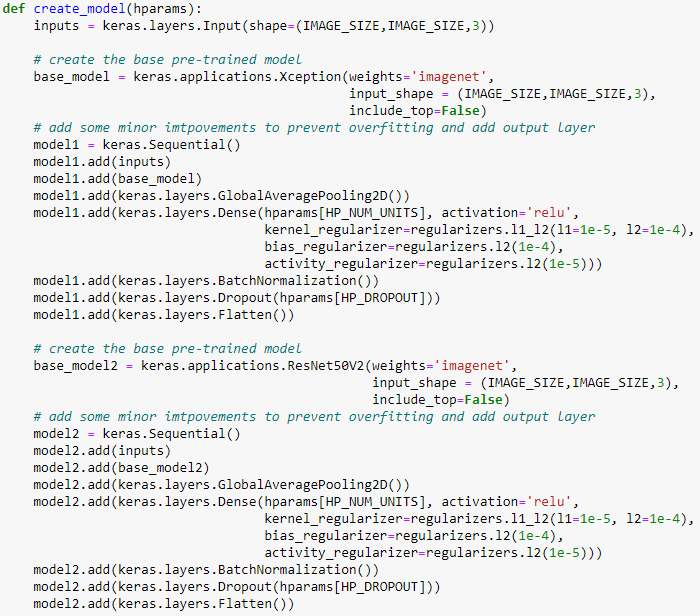
\includegraphics[width=\textwidth]{figures/xception-improvement-3-part1.png}
    \caption{The first half of the Xception-ResNet50V2 model.}
    \label{fig:xception-improvement-3-part1}
\end{figure}
\begin{figure}[H]
    \centering
    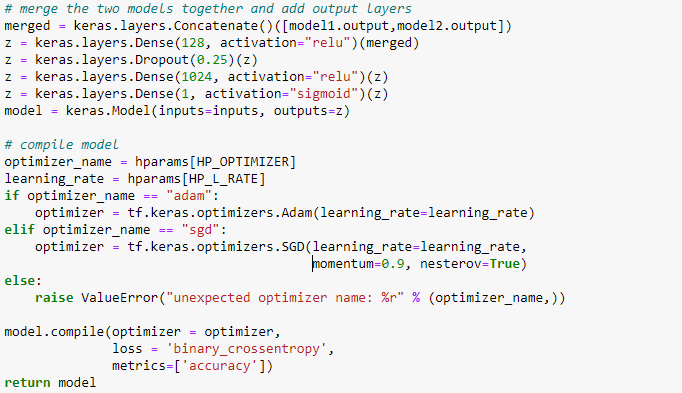
\includegraphics[width=\textwidth]{figures/xception-improvement-3-part2.png}
    \caption{The second half of the Xception-ResNet50V2 model.}
    \label{fig:xception-improvement-3-part2}
\end{figure}
\begin{figure}[H]
    \centering
    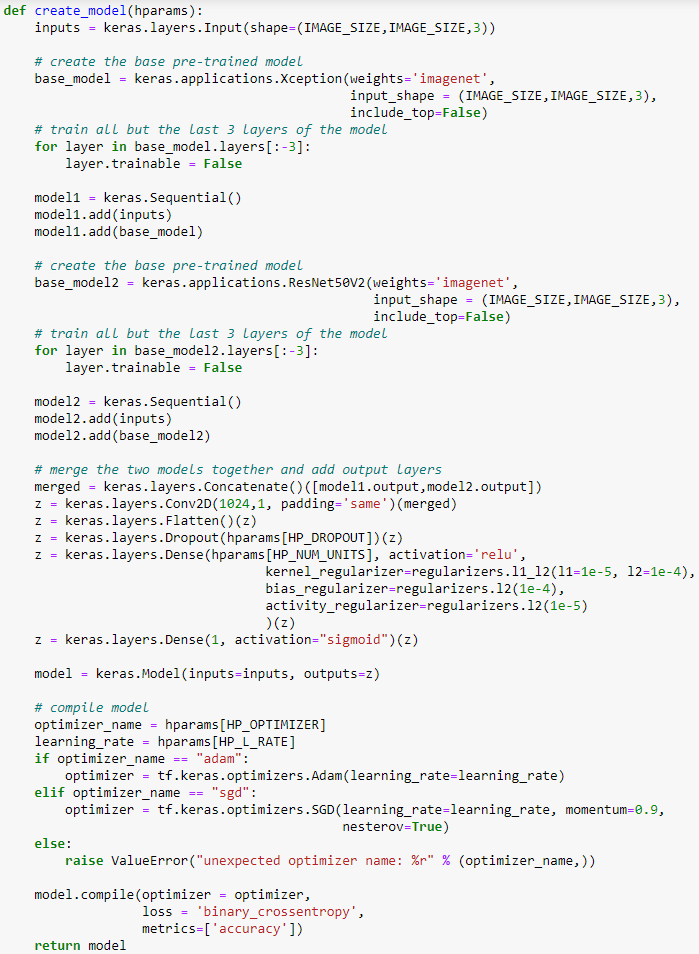
\includegraphics[width=\textwidth]{figures/xception-improvement-4.png}
    \caption{The second version of the Xception-ResNet50V2 model.}
    \label{fig:xception-improvement-4}
\end{figure}
\begin{figure}[H]
    \centering
    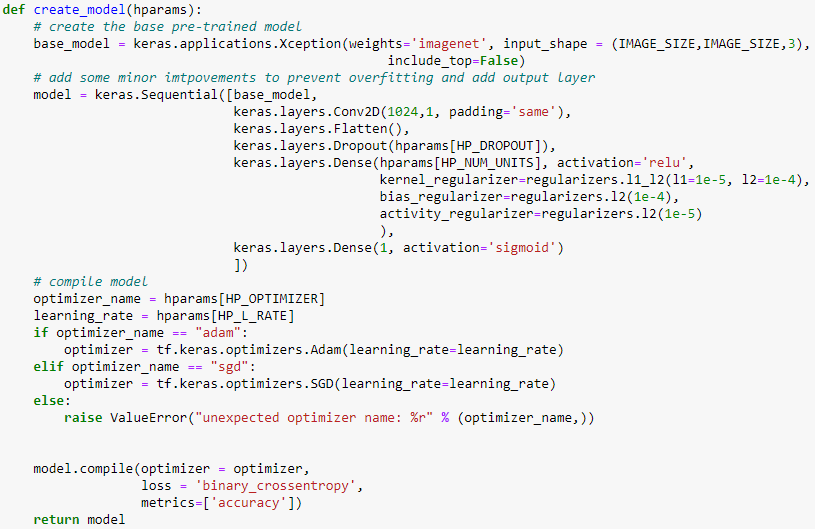
\includegraphics[width=\textwidth]{figures/xception-improvement-5.png}
    \caption{The final improvement to the Xception model.}
    \label{fig:xception-improvement-5}
\end{figure}

\begin{landscape}
\begin{table}
    \caption{Xception improvements results after training on the small COVIDx-CXR dataset.}
    \centering
    \begin{tabular}{l|l|l|l|l|l|l|l|l|l|l}
    Model & \begin{tabular}[c]{@{}l@{}}Dense\\ Units\end{tabular} & Dropout & Optimiser & \begin{tabular}[c]{@{}l@{}}Learning\\ Rate\end{tabular} & \begin{tabular}[c]{@{}l@{}}Mean \\ Validation \\ Accuracy\end{tabular} & \begin{tabular}[c]{@{}l@{}}Best Fold \\ Test \\ Accuracy\end{tabular} & \begin{tabular}[c]{@{}l@{}}Mean Test\\ Precision\end{tabular} & \begin{tabular}[c]{@{}l@{}}Mean Test\\ Recall\end{tabular} & \begin{tabular}[c]{@{}l@{}}Mean Test\\ F1 Score\end{tabular} & \begin{tabular}[c]{@{}l@{}}Mean \\ Training\\ Time (s)\end{tabular} \\
    Improvement 1 & 128 & 0.1 & Adam & 0.001 & 0.6827 & 0.6325 & 0.7293 & 0.2780 & 0.3600 & 177 \\
    Improvement 1 & 128 & 0.1 & \begin{tabular}[c]{@{}l@{}}SGD \& \\ Momentum\end{tabular} & 0.001 & 0.6180 & 0.6225 & 0.5903 & 0.1510 & 0.2241 & 187 \\
    Improvement 2 & 128 & 0.1 & Adam & 0.001 & 0.9527 & 0.9800 & 0.9837 & 0.8950 & 0.9331 & 1132 \\
    Improvement 2 & 128 & 0.1 & \begin{tabular}[c]{@{}l@{}}SGD \& \\ Momentum\end{tabular} & 0.001 & 0.9253 & 0.8975 & 0.9316 & 0.7920 & 0.8555 & 1200 \\
    Improvement 3 & 128 & 0.1 & Adam & 0.001 & 0.9407 & 0.9775 & 0.9864 & 0.8310 & 0.8915 & 1389 \\
    Improvement 4 & 128 & 0.1 & Adam & 0.001 & 0.9465 & 0.9325 & 0.7787 & 0.6660 & 0.7177 & 646 \\
    Improvement 5 & 128 & 0.1 & Adam & 0.001 & 0.7180 & 0.9375 & 0.6826 & 0.5590 & 0.5161 & 922
    \end{tabular}
    \label{fig:xception-improvement-results}
\end{table}
\end{landscape}